%%
%% This is file `sample-sigplan.tex',
%% generated with the docstrip utility.
%%
%% The original source files were:
%%
%% samples.dtx  (with options: `sigplan')
%% 
%% IMPORTANT NOTICE:
%% 
%% For the copyright see the source file.
%% 
%% Any modified versions of this file must be renamed
%% with new filenames distinct from sample-sigplan.tex.
%% 
%% For distribution of the original source see the terms
%% for copying and modification in the file samples.dtx.
%% 
%% This generated file may be distributed as long as the
%% original source files, as listed above, are part of the
%% same distribution. (The sources need not necessarily be
%% in the same archive or directory.)
%%
%% Commands for TeXCount
%TC:macro \cite [option:text,text]
%TC:macro \citep [option:text,text]
%TC:macro \citet [option:text,text]
%TC:envir table 0 1
%TC:envir table* 0 1
%TC:envir tabular [ignore] word
%TC:envir displaymath 0 word
%TC:envir math 0 word
%TC:envir comment 0 0
%%
%%
%% The first command in your LaTeX source must be the \documentclass command.
\documentclass[sigplan,screen]{acmart}
%% NOTE that a single column version is required for 
%% submission and peer review. This can be done by changing
%% the \doucmentclass[...]{acmart} in this template to 
%% \documentclass[manuscript,screen,review]{acmart}
%% 
%% To ensure 100% compatibility, please check the white list of
%% approved LaTeX packages to be used with the Master Article Template at
%% https://www.acm.org/publications/taps/whitelist-of-latex-packages 
%% before creating your document. The white list page provides 
%% information on how to submit additional LaTeX packages for 
%% review and adoption.
%% Fonts used in the template cannot be substituted; margin 
%% adjustments are not allowed.
%%
%% \BibTeX command to typeset BibTeX logo in the docs
%  \AtBeginDocument{%
%   \providecommand\BibTeX{{%
%      \normalfont B\kern-0.5em{\scshape i\kern-0.25em b}\kern-0.8em\TeX}}}

%% Rights management information.  This information is sent to you
%% when you complete the rights form.  These commands have SAMPLE
%% values in them; it is your responsibility as an author to replace
%% the commands and values with those provided to you when you
%% complete the rights form.
% \setcopyright{acmcopyright}
% \copyrightyear{2018}
% \acmYear{2018}
% \acmDOI{XXXXXXX.XXXXXXX}

%% These commands are for a PROCEEDINGS abstract or paper.
% \acmConference[Conference acronym 'XX]{Make sure to enter the correct
%   conference title from your rights confirmation emai}{June 03--05,
%   2018}{Woodstock, NY}
%
%  Uncomment \acmBooktitle if th title of the proceedings is different
%  from ``Proceedings of ...''!
%
%\acmBooktitle{Woodstock '18: ACM Symposium on Neural Gaze Detection,
% %  June 03--05, 2018, Woodstock, NY} 
% \acmPrice{15.00}
% \acmISBN{978-1-4503-XXXX-X/18/06}
\usepackage{parskip}


%%
%% Submission ID.
%% Use this when submitting an article to a sponsored event. You'll
%% receive a unique submission ID from the organizers
%% of the event, and this ID should be used as the parameter to this command.
%%\acmSubmissionID{123-A56-BU3}

%%
%% For managing citations, it is recommended to use bibliography
%% files in BibTeX format.
%%
%% You can then either use BibTeX with the ACM-Reference-Format style,
%% or BibLaTeX with the acmnumeric or acmauthoryear sytles, that include
%% support for advanced citation of software artefact from the
%% biblatex-software package, also separately available on CTAN.
%%
%% Look at the sample-*-biblatex.tex files for templates showcasing
%% the biblatex styles.
%%

%%
%% The majority of ACM publications use numbered citations and
%% references.  The command \citestyle{authoryear} switches to the
%% "author year" style.
%%
%% If you are preparing content for an event
%% sponsored by ACM SIGGRAPH, you must use the "author year" style of
%% citations and references.
%% Uncommenting
%% the next command will enable that style.
%%\citestyle{acmauthoryear}

%%
%% end of the preamble, start of the body of the document source.
\begin{document}

%%
%% The "title" command has an optional parameter,
%% allowing the author to define a "short title" to be used in page headers.
\title{Deadlock Detection, Prevention, and Avoidance}

%%
%% The "author" command and its associated commands are used to define
%% the authors and their affiliations.
%% Of note is the shared affiliation of the first two authors, and the
%% "authornote" and "authornotemark" commands
%% used to denote shared contribution to the research.
\author{Samridh Agarwal(20BIT0402)}
% \email{samridh.agarwal2020@}
% \orcid{1234-5678-9012}
\author{Sanchit Sandeep Khedkar(20BIT0406)}
\author{Astha Jha(20BIT0268)}
\author{Bhavya Saini(20BIT0020)}
\author{Anish Mittal(20BIT0343)}
\author{Vidoosh Bang(20BIT0318)}
\author{Parthvi Singh(20BIT0377)}
\author{Ananya Grover(20BIT0176)}
\author{Pranav Desai(20BIT0167)}
\author{Megha Maitin(20BIT0177)}
\author{Rahul Jamdade(20BIT0279)}
\author{Karan Ravi(20BIT0162)}
\author{Ishani Chowdhury(20BIT0175)}



%%
%% By default, the full list of authors will be used in the page
%% headers. Often, this list is too long, and will overlap
%% other information printed in the page headers. This command allows
%% the author to define a more concise list
%% of authors' names for this purpose.
% \renewcommand{\shortauthors}{Trovato and Tobin, et al.}

%%
%% The abstract is a short summary of the work to be presented in the
%% article.
\begin{abstract}
A deadlock is a situation where more than two processes are blocked because each process is holding a resource that is essential and is waiting for another resource which has been acquired by another process. The following text goes though existing literature to find optimal solutions to existing problems pertaining to deadlocks.
\end{abstract}

%%
%% The code below is generated by the tool at http://dl.acm.org/ccs.cfm.
%% Please copy and paste the code instead of the example below.
%%
% \begin{CCSXML}
% <ccs2012>
%  <concept>
%   <concept_id>10010520.10010553.10010562</concept_id>
%   <concept_desc>Computer systems organization~Embedded systems</concept_desc>
%   <concept_significance>500</concept_significance>
%  </concept>
%  <concept>
%   <concept_id>10010520.10010575.10010755</concept_id>
%   <concept_desc>Computer systems organization~Redundancy</concept_desc>
%   <concept_significance>300</concept_significance>
%  </concept>
%  <concept>
%   <concept_id>10010520.10010553.10010554</concept_id>
%   <concept_desc>Computer systems organization~Robotics</concept_desc>
%   <concept_significance>100</concept_significance>
%  </concept>
%  <concept>
%   <concept_id>10003033.10003083.10003095</concept_id>
%   <concept_desc>Networks~Network reliability</concept_desc>
%   <concept_significance>100</concept_significance>
%  </concept>
% </ccs2012>
% \end{CCSXML}

% \ccsdesc[500]{Computer systems organization~Embedded systems}
% \ccsdesc[300]{Computer systems organization~Redundancy}
% \ccsdesc{Computer systems organization~Robotics}
% \ccsdesc[100]{Networks~Network reliability}

%%
%% Keywords. The author(s) should pick words that accurately describe
%% the work being presented. Separate the keywords with commas.
% \keywords{datasets, neural networks, gaze detection, text tagging}

%% A "teaser" image appears between the author and affiliation
%% information and the body of the document, and typically spans the
%% page.
% \begin{teaserfigure}
%   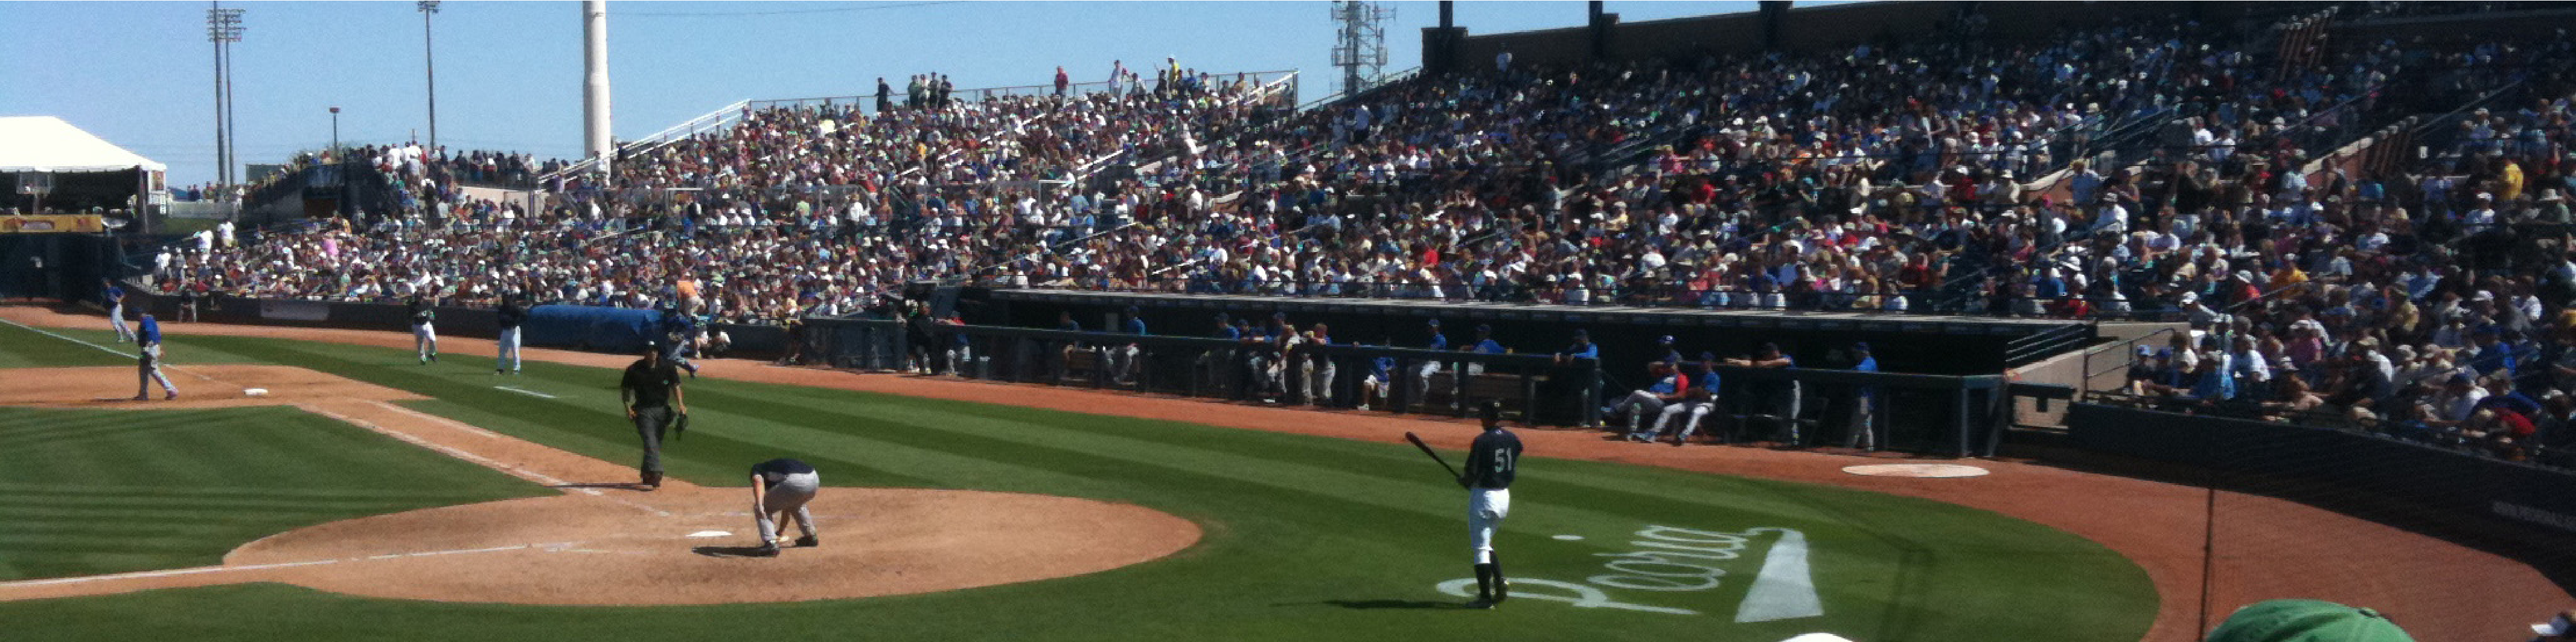
\includegraphics[width=\textwidth]{sampleteaser}
%   \caption{Seattle Mariners at Spring Training, 2010.}
%   \Description{Enjoying the baseball game from the third-base
%   seats. Ichiro Suzuki preparing to bat.}
%   \label{fig:teaser}
% \end{teaserfigure}

%%
%% This command processes the author and affiliation and title
%% information and builds the first part of the formatted document.
\maketitle

\section{Introduction}
Deadlock prevention techniques the critical section is mainly considered in mutual exclusion where deadlock occurs, so to prevent this situation we have implemented the prevention algorithm of mutual exclusion. Considering a similar scenario we have also implemented a hold and wait and no-preemption prevention algorithm. In circular wait, the processes are blocked in a loop which creates a deadlock situation where they cannot access any other resources. To prevent this situation we have implemented a circular wait prevention algorithm. 

A deadlock is a situation where multiple program/process are sharing a common resource and are preventing each other from accessing the resource and are waiting for each other to release the resource in order to progress any further. Deadlock detection is necessary as when a deadlock occurs it will completely halt the ongoing process until the required resource is not released or the program gets terminated. Deadlock can occur if and only if all of these 4 conditioned are fulfilled: 1. Mutual Exclusion: The resources involved must be unshareable; otherwise, the processes would not be prevented from using the resource when necessary. 2. Hold and Wait: Requesting process hold already, resources while waiting for requested resources. 3. No Preemption: Resources already allocated to a process cannot be preempted. 4. Circular Wait: The processes in the system form a circular list or chain where each process in the list is waiting for a resource held by the next process in the list.
 The probability of deadlocks depends on factors such as process mix, resource request and release patterns, resource holding time, and the average number of data objects held (locked) by processes. The probability of deadlocks is difficult to analyze because deadlock occurrence is highly sensitive to the timing and order in which resource requests are made. There is always a need of improvement in software algorithms because we are processing more and more data. Algorithm improvements are important even if its only a small improvement.
 \section{Literature Review}
 \\
 A Deadlock Prevention Policy for a Class of Multithreaded Software; Wenli Duo, et al. study the problem of deadlock prevention in a class of ordinary Gadara nets, which are a subclass of Petri nets proposed by Wang et al. Compared with other subclasses of Petri nets, it better models concurrent programs with lock acquisition and release operations. An iterative control scheme based on siphons is proposed to obtain a maximally permissive supervisor with a small number of monitor places. They begin by defining Petri nets, siphons, Gadara nets, and controlled Gadara nets. They then go on to provide a method on bad markings based on siphons and state that deadlocks are closely related to emptiable siphons in Gadara nets; specifically, a net system is non-live once a siphon is emptied. They note that random control of siphons in Gadara nets leads to high computational complexity if the number of siphons controlled is very large, and emergence of bad siphons whose control is complex than emptiable siphons is possible. They then go on to define a live marking, a bad marking, a deadlock marking in a Petri net, noting that a marking is bad if it can reach deadlock markings via a branching transition since it cannot be controlled by monitors. A method of obtaining bad markers is then shown based on a function FindBM. Minimum resource number emptiable siphon MRNE is required to be computed for bad markings to be computed by FindBM, which is computed by function ComputeMRES. They then propose an iterative deadlock prevention policy to obtain a live Gadara net, which they then apply to two Gadara nets. The first example shows that the proposed method guarantees the liveness of Gadara nets with maximal permissiveness in three iterations of the algorithm.  For the second example, there are four iterations and four constraints are constructed by the algorithm and each of them corresponds to a monitor place. After adding these four monitor places to the original Gadara net, the controlled net is live with 11 live markings. The computational complexity of the proposed approach is in theory exponential since it requires enumerating all or part of reachable markings. Another limitation is that the approach is applicable to a class of ordinary Gadara nets only, where each idle place contains exactly one token at the initial marking.
\par
Deadlock Free Resource Management Technique For Iot-Based Post Disaster Recovery Systems; Madhavi Devi B, et al. talk about an IoT based network to aid in disaster recovery and addresses the problem of resource allocation and management by attempting to re investigate the resource reservation policies to answer the question of “How many resources must be reserved and how they must be allocated to avoid deadlock completely?”. They take a look at existing literature and provide an overview of what they aimed to solve. They then go on to describe a post disaster management system resource pool. They then go on to analyse existing techniques of deadlock avoidance with motivational examples, then go on to propose Deadlock Free Resource Reservation Techniques to ensure that deadlock will never occur. It suggests to reserve some resources in the reservation and the remaining resources are made available in the available pool. Whenever a process requests for a set of resources, available pool resources are granted. In case the request cannot be granted only from the available pool then the reservation pool are also used such that the maximum resources this process can ever want are granted to give this process the chance to complete. They simulate the proposed techniques on a 2.0GHz processor and find that average turnaround time is approximately 18\% lower for the proposed techniques than Banker’s algorithm.
\par
A Deflection-Based Deadlock Recovery Framework to Achieve High Throughput for Faulty NoCs; Yibo Wu, et al. say that deadlocks on Network-on-Chip (NoC) is a severe problem because conventional problems on deadlock freedom are unavailable on NoCs. A Deflection Based Deadlock Recovery (DBDR) framework is proposed to achieve high over-saturation throughput and fairness for faulty NoCs. They take a look at existing deadlock recovery approaches and find that over saturation throughput is significant for them, along with finding a positive feedback loop between deadlocks and congestions that can amplify the negative impact of the reasons for deadlock based recovery approaches, which form the basis of DBDR design. They propose a deadlock recovery framework that handles congestions and deadlocks in the same framework. The proposed recovery method combines probe detection and timeout counters to achieve an accurate and timely deadlock detection. DBDR goes into a deflection mode upon detection of potential deadlock and routes and ejects all packets with high efficiency; it is topology agnostic  and achieves full adaptive routing  and deadlock freedom. They present a distributed implementation to make the entire network enter and exit the deflection mode The implementation is done by broadcasting a triggering message and an empty signal via a bufferless subnetwork, and using a onebit wire grid to finish the deflection mode. The experimental results demonstrate that under real workloads, DBDR can reduce the average latency by up to 50\%.
\par
Deadlock detection in distributed system; Kshirod Kumar Rout, et al.  propose a deadlock detection algorithm using C++ and Python; and found that the mechanism worked fine for different sections of a distributed system. The performance of the system was measured in terms of time, space, number of messages sent and received. It gave an idea about how resources were allocated, and how few processes resulted in a deadlock state.
\\
Research method used-
\newline
The proposed algorithm for the detection of deadlock is explained in detail below. Here C++ and python are used as the programming language.
\begin{itemize}
\item Step 1: We have simulated software that is used to detect the deadlock in an office environment. The operator of the software is a resource administrator and checks for the availability of resources based on the resources available at the current time.
\item Step 2: There are multiple instances of resources available in the office and there are 4 employees in the office using the resources.
\item Step 3: They are requesting the use of resources at any given time which the administrator knows and enters as input to the software.
\item Step 4: The software at that time randomly distributes the resources, i.e., the resources on hold by employees based on the total number of resources available. We have used rand() to randomly distribute the resources among the employees.
\item Step 5: After that, we calculate the resources available and take the resources requested by users as input and check for the possibility of assigning the resources by taking counters if the resources requested by a particular person is less, i.e., the number of printers, scanners, tape drive, fax then the counter value is increased till 4. If the counter value turns out to be 4 then resources are assigned to the person and the total resources available at that time are added upon by the person’s resources in the available matrix. If the counter does not go up to 4 in any case then deadlock is detected.
\item Step 6: Now coming to different matrices we have used:
a) fraction[]: It is used for randomly storing the number of resources allocated at any time.
b) request[]: It is used for storing the resources requested by users at any time.
c) srand[]: It is used for generating a seed at a particular time otherwise if we use rand() in C++ directly then it will always return the same random numbers after executing multiple times. So by using srand() we will be generating random numbers.
d) available[]: It is used to check for the resources available by subtracting the total number of resources available with the total number of resources on hold.
\end{itemize}
\par
A Survey on Deadlock Detection Algorithms for Distributed Systems; Mega Putra et al. discuss deadlock detection in distributed systems and claim that deadlock detection and resolution is complex for distributed systems as several sites gets affected and nodes often are note aware of the other sites or processes responsible for deadlock. Distributed deadlock detection is also difficult because of the lack of a common global memory for all the different sites of the network. They discuss four algorithms and compare the time-space complexity of the four, information on deadlock after detection, and problems faced by the algorithms. They then go on to highlight improvements over the years by more recent algorithms.
\par
An Experimental Execution Of Deadlock Algorithms; Karthik Konar, et al. implement techniques such as Mutual Exclusion, Hold and Wait, No-Preemption, Circular Wait, Process Termination, Roll Back, Selecting a Victim, and Starvation. The typical method of resolving the deadlock is to select the victim and abort that process Another than that process termination and rollback are also the two resolution methods wherein termination of the process every process is been terminated to resolve the deadlock situation and in rollback, the processes are been rolled back till the point where the deadlock had been occurred. Starvation is also one of the deadlock recovery techniques which mainly focuses on the process which has the lowest priority. Deadlock prevention techniques the critical section is mainly considered in mutual exclusion where deadlock occurs, so to prevent this situation they have implemented the prevention algorithm of mutual exclusion. Considering a similar scenario they have also implemented hold and wait and no-preemption prevention algorithm. In circular wait, the processes are been blocked in a loop which creates a deadlock situation where they cannot access any other resources to prevent this situation they have implemented a circular wait prevention 
\par
Approaches for deadlock detection for distributed systems:
Deadlock detection necessitates a review of the state of process-resource interactions to see if there are any cyclic interactions.
The discovery of deadlocks in distributed systems appears to be a difficult task.
The basic approach for detecting distributed deadlock is as follows:
Create the local wait for graph (WFG), Add possible edges
obtained from other sites that may cause deadlock, The local
WFG now also contains locks on remote objects and the sub
transaction holding those lock, Determine the cycles, if it is
to be found. There is a deadlock.
\par
Path-pushing algorithms: Under this class of algorithm, some simplified form of global WFG is built at each site. Each site sends its local WFG to a number of neighbouring sites every time a deadlock computation is performed. After the updation of the local data structure, the updated WFG is passes along and the procedure is repeated until some site has the complete picture of the global situation to announce as to if the deadlock is present or not. 
\par
Edge- chasing algorithms: With the help of propagating special messages called probes, the presence of a cycle in a distributed graph structure can be verified. Probes are distinct from resource request and grant messages. When the initiator of such a probe
computation receives a matching probe, it knows that it is in cycle in the graph. Blocked processes propagate the probe along their
outgoing edges. 
\par
Distributed deadlock prevention: Each transaction must lock its complete data item before it can begin execution, according to the techniques. They demand that all data items be partially ordered, and that a transaction can only lock data items in the order defined by the partial order.
Designing a system so that deadlock is impossible is an alternative to detecting deadlocks. Obtaining a global timestamp for each transaction (such that no two transactions have the same timestamp) is one technique to accomplish this. Check which of the two processes has a younger timestamp and give priority to the older process when one process is going to block waiting for a resource that another process is consuming.
If the resource is being used by a younger process, the older process (which needs the resource) must wait. If the resource is held by an older process, the younger process (which seeks the resource) kills itself. This pushes the graph of resource utilisation to be steered from older to younger operations, effectively eliminating cycles. This algorithm is known as the wait-die algorithm.
\par
Approaches for Deadlock Detection and Deadlock Prevention for Distributed system, Dhiraj Gupta, Gupta V,K found the following-
Approaches for deadlock detection for distributed systems:
Deadlock detection necessitates a review of the state of process-resource interactions to see if there are any cyclic interactions.
The discovery of deadlocks in distributed systems appears to be a difficult task.
The basic approach for detecting distributed deadlock is as follows:
Create the local wait for graph (WFG), Add possible edges
obtained from other sites that may cause deadlock, The local
WFG now also contains locks on remote objects and the sub
transaction holding those lock, Determine the cycles, if it is
to be found. There is a deadlock.
\\
Path-pushing algorithms: Under this class of algorithm, some simplified form of global WFG is built at each site. Each site sends its local WFG to a number of neighbouring sites every time a deadlock computation is performed. After the updation of the local data structure, the updated WFG is passes along and the procedure is repeated until some site has the complete picture of the global situation to announce as to if the deadlock is present or not. 
\\
Edge- chasing algorithms: With the help of propagating special messages called probes, the presence of a cycle in a distributed graph structure can be verified. Probes are distinct from resource request and grant messages. When the initiator of such a probe
computation receives a matching probe, it knows that it is in cycle in the graph. Blocked processes propagate the probe along their
outgoing edges. 
\\
Distributed deadlock prevention: Each transaction must lock its complete data item before it can begin execution, according to the techniques. They demand that all data items be partially ordered, and that a transaction can only lock data items in the order defined by the partial order.
Designing a system so that deadlock is impossible is an alternative to detecting deadlocks. Obtaining a global timestamp for each transaction (such that no two transactions have the same timestamp) is one technique to accomplish this. Check which of the two processes has a younger timestamp and give priority to the older process when one process is going to block waiting for a resource that another process is consuming.
If the resource is being used by a younger process, the older process (which needs the resource) must wait. If the resource is held by an older process, the younger process (which seeks the resource) kills itself. This pushes the graph of resource utilisation to be steered from older to younger operations, effectively eliminating cycles. This algorithm is known as the wait-die algorithm.
\par
The Tick Formulation for deadlock detection and avoidance in railways traffic control; Vernonica Del Sasso, et al.-
If and only if it is not possible to construct a conflict-free plan that routes the trains to their destinations, a group of trains is said to be bound-to-deadlock. Assume you discover a train that can travel from point A to point B without colliding with other trains while simultaneously holding all of the other n-1 trains at their points of origin. Rather than identifying one or more culprit sets, this method will find a tripartition Q, C, P of the set M of trains such that: the trains in Q can still continue running to their destination; the trains in C will be halted in their current position, waiting for recovery actions to solve the deadlock; the trains P cannot reach their destination because of the trains in C, but they should not be considered responsible for the deadlock because they can be parked in suitable sags; and the trains P If a train must wait for the railway paths to be cleared by other trains, it may remain stationary for several ticks. The number of boundary nodes and black holes created depends on the trains involved: if a train's timetable terminates at a yard in the middle of the single-tracked line under investigation, a black hole is inserted to allow the train to continue on its original itinerary without becoming trapped in the tested region. No train has to wait for another train in the most optimistic situation, and the lower bound on T can be set to the maximum number of moves that the farthest train must make to reach its black hole. Train A must stop at the first station and wait for train B for 8 ticks, requiring at least 18 ticks to route both trains over the network. For each m∉M, we denote by Am∈A the subset of route arcs feasible for train m and with p(m, a)⊆Am (resp. f(m,a)), reachable by m. δ−(s)m denotes the set of route arcs incoming the stopping node s in V that can be traversed by train m. Allowing dummy trains to traverse the network is a possible safe place assignment for a subset of trains in M, which can be derived from the route arcs occupied by trains at tick T. Constraints specify how trains travel on the network and how dummy trains are handled so that trains can be parked in legal and safe locations. We avoid generating superfluous variables for trains in M and ticks in [T] by noting that the matching variable at tick T will have the same value. We define for each M× A× [T] and M' A [T'] variables xm,a,t for the head of the train. Let A ‘ be the set of all possible sets A’ : 
\begin{figure}
    \centering
    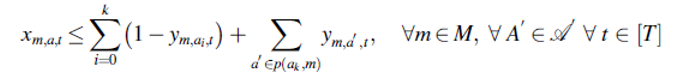
\includegraphics[width=\linewidth]{1.png}
\end{figure}

Note that, as the route for any train m is not fixed, we write constraints for each subset A whose routes are not long enough to fit the whole train.
No-swap constraints: a route arc occupied by a train at tick t cannot be occupied by a train in the opposite direction at tick t+1.
At the final tick, each train m must be placed at a route arc belonging to one of the following three subsets: the black holes(Bm), the set of safe places(Sm), the initial position of train m. Constraints ensure trains are stopped at their initial position whenever hm = 1: 
\begin{figure}[h]
    \centering
    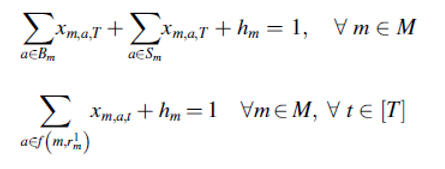
\includegraphics[width=\linewidth]{2.png}
\end{figure}

The following sets of constraints describe the movements of dummy trains at ticks [T]. 
\begin{itemize}
    \item dummy trains originates at a black hole:
 \begin{figure}[h]
    \centering
    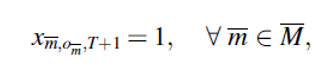
\includegraphics[width=\linewidth]{3.png}
\end{figure}
\item each dummy tick, each dummy train’s head is allocated to exactly one of its feasible routes:
 \begin{figure}[h]
    \centering
    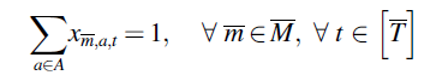
\includegraphics[width=\linewidth]{4.png}
\end{figure}
\item at each dummy tick, a dummy train can only move forward (22), unless it already reached its final black hole (23):
 \begin{figure}[h]
    \centering
    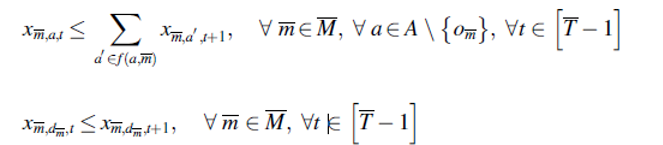
\includegraphics[width=\linewidth]{5.png}
\end{figure}
\item At each dummy tick, dummy trains cannot occupy route arcs incompatible with the ones occupied by trains in safe places:
 \begin{figure}[h]
    \centering
    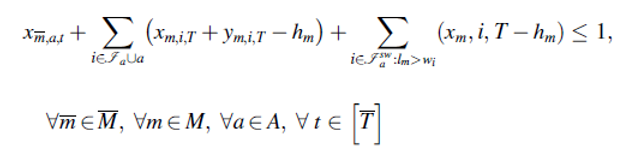
\includegraphics[width=\linewidth]{6.png}
\end{figure}

Since tick t+1 can start only after each train m ∈ Mt reached the stopping point am,t+1 , we can use the following formula:
 \begin{figure}[h]
    \centering
    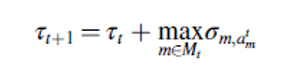
\includegraphics[width=\linewidth]{7.png}
\end{figure}
\end{itemize}
to calculate the starting time of all ticks t = 2,… , T. Then, at time τt , each train in m ∈ Mt moves from am,t to am,t+1. As deadlocks are most frequently caused by a small number of trains, we focused on instances with up to 7 trains.
The greatest number of such subsets is equal to the sum of each train's number of moves, however this is frequently a superfluous quantity that just adds to the formulation's size and computational time. With respect to the number of trains and network dimension, the formulation is polynomial. The difficulty in determining the proper parameter for the number of ticks remains the formulation's fundamental flaw. As a result, we're looking into ways to address the deadlock detection problem and alternative formulations.
\par
Collision-Free Trajectory Planning With Deadlock Prevention: An Adaptive Virtual Target Approach; Rishi Mohan, et al.-
\\
Most human-centred robotic applications require robots to follow a certain pre-defined path. This makes the robot's autonomous movements acceptable and predictable for humans. Planning a trajectory for the robot thus involves guiding it along this desired path. 
This chapter presents a novel approach for trajectory planning in which an Adaptive Virtual Target (AVT) is formulated that follows the desired path irrespective of surrounding obstacles. The AVT essentially plays the role of a moving reference for the trajectory planner to track. Additionally, the AVT velocity can be adapted such that the robot can catch up in case of deviations from the path due to obstacle avoidance manoeuvres.
The proposed approach allows the robot to keep moving towards the goal by preventing deadlocks while simultaneously minimizing deviation from the desired path. Simulations based on a medical X-ray robot are provided to validate the approach.
\begin{itemize}
\item A. Virtual Target Formulation
Assuming a path is defined by waypoints, a deadlock occurs when the robot is faced with the contradictory objectives of reaching a waypoint while trying to avoid a collision with an obstacle which is blocking this waypoint. The crux of this paper is a waypoint independent approach which eliminates the occurrence of this contradiction. To this end, a virtual target is formulated which is constrained to travel along the desired path irrespective of the surrounding obstacles. This virtual target can be thought of as a dynamic waypoint which serves as a moving reference point to be tracked by the actual robot. Under assumption, this approach ensures the existence of a reference point which is not blocked by an obstacle for infinite time and guides the robot along a desired path towards its goal.

The virtual target is modelled as a wheeled mobile robot which moves along P(s) according to
x˙v(s)=Vcosθv(s)
y˙v(s)=Vsinθv(s)
θv(s)=Vκ(s)

V is virtual target’s linear velocity and yv=[xvyvθv] is the configuration (position and heading) of the virtual target which effectively yields the reference for the actual robot.

The virtual target does not account for the kinematics and/or dynamics of the actual robot and is not restricted by any constraints to avoid collision

\item B. Adaptive Velocity Function
The choice of  V is a design parameter to be chosen by the user. Although a constant value of  V would serve the purpose of a moving virtual target which guides the actual robot towards the final goal, it does not account for any deviations between the position of the target and robot. Since the robot is constrained to follow the preceding AVT, in case of a curved path or a large deviation (due to obstacle avoidance) the phenomenon of ‘corner cutting’ is observed. This behaviour escalates with increasing deviation from the AVT . To this end, instead of choosing a constant V, an adaptive velocity function based on  is formulated as
V=Vd(1−ηtanh(γ))
where Vd>0 is the fixed AVT velocity, 0<η<1 is a constant and 
γ is the euclidean distance between the AVT and the actual robot. The function provides AVT with the capability to slow down when the robot is far away from P(s) and the strength of the function to reduce AVT velocity depends on parameter η.
Remark 2:
The condition 0<η<1ensures that the virtual target does not
move backwards along the path (V<0) ensuring a forward moving reference progressing towards the goal and not away from it;
come to a complete halt (V = 0) resulting in a deadlock. Although, η≈1 does cause the AVT to move extremely slowly when γ is large.
\end{itemize}
\begin{itemize}
\item A. Deadlock Example
To provide a baseline for comparison, consider the example in where the desired path (yellow) is segmented into three waypoints (red circles) which the robot must track to follow the desired path (robot geometry is omitted for clarity). The obstacle O1(white square) is placed (after waypoint generation) such that it completely envelopes the second waypoint. Using the MPC-based planner in, a trajectory is generated from start (blue circle) towards the goal (green circle). The generated trajectory (blue) tracks the first waypoint, however it is constrained to avoid the obstacle while trying to reach the second waypoint. This creates a deadlock situation rendering the robot stationary around the waypoint without ever reaching it. also depicts the longitudinal (x) and lateral (y) coordinates which remain unchanged after t=40, thus resulting in a stationary robot for infinite time.
\begin{figure}[h]
    \centering
    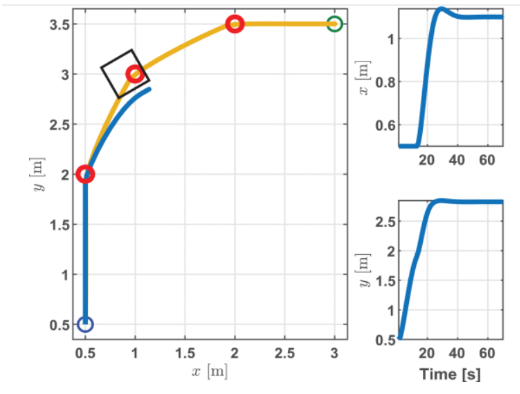
\includegraphics[width=\linewidth]{8.png}
\end{figure}
\item B. Deadlock Prevention - AVT Approach
Trajectory planning based on the proposed ATV approach is compared to the baseline example described above. Consider the scenario in Fig. 5, where Rneeds to move from its starting configuration, x0(blue circle), to its final configuration, xf(green circle) along the desired path (yellow). The static obstacle O1(purple) intersects the path of Rpresents the MPC-based collision-free trajectory (black curve) generated using a constant velocity virtual target, i.e., η=0 in. In, the resultant trajectory (grey curve) is based on a virtual target with adaptive velocity (η>0). For both cases a collision-free trajectory is successfully planned from initial to final configuration, illustrating the prevention of a deadlock as compared to the baseline example. Time stamps of the virtual target (blue triangle) at t∈{6.25,11.25,14.5,20.25}in both cases show that the AVT moves along P(s)irrespective of O1, thereby ensuring an obstacle-free reference point for the MPC-planner to track.
\begin{figure}[h]
    \centering
    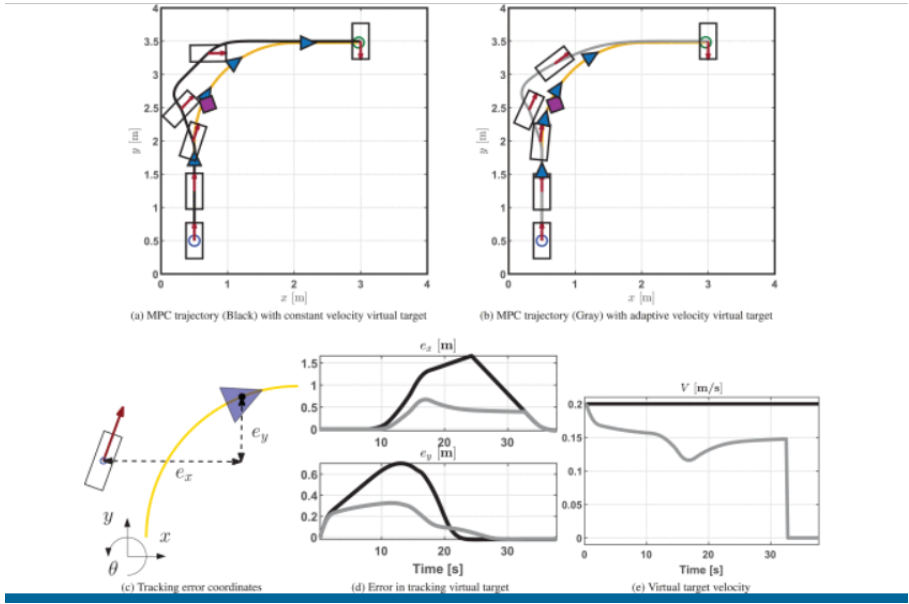
\includegraphics[width=\linewidth]{9.png}
\end{figure}
\end{itemize}


% \section{Template Overview}
% As noted in the introduction, the ``\verb|acmart|'' document class can
% be used to prepare many different kinds of documentation --- a
% double-blind initial submission of a full-length technical paper, a
% two-page SIGGRAPH Emerging Technologies abstract, a ``camera-ready''
% journal article, a SIGCHI Extended Abstract, and more --- all by
% selecting the appropriate {\itshape template style} and {\itshape
%   template parameters}.

% This document will explain the major features of the document
% class. For further information, the {\itshape \LaTeX\ User's Guide} is
% available from
% \url{https://www.acm.org/publications/proceedings-template}.

% \subsection{Template Styles}

% The primary parameter given to the ``\verb|acmart|'' document class is
% the {\itshape template style} which corresponds to the kind of publication
% or SIG publishing the work. This parameter is enclosed in square
% brackets and is a part of the {\verb|documentclass|} command:
% \begin{verbatim}
%   \documentclass[STYLE]{acmart}
% \end{verbatim}

% Journals use one of three template styles. All but three ACM journals
% use the {\verb|acmsmall|} template style:
% \begin{itemize}
% \item {\verb|acmsmall|}: The default journal template style.
% \item {\verb|acmlarge|}: Used by JOCCH and TAP.
% \item {\verb|acmtog|}: Used by TOG.
% \end{itemize}

% The majority of conference proceedings documentation will use the {\verb|acmconf|} template style.
% \begin{itemize}
% \item {\verb|acmconf|}: The default proceedings template style.
% \item{\verb|sigchi|}: Used for SIGCHI conference articles.
% \item{\verb|sigchi-a|}: Used for SIGCHI ``Extended Abstract'' articles.
% \item{\verb|sigplan|}: Used for SIGPLAN conference articles.
% \end{itemize}

% \subsection{Template Parameters}

% In addition to specifying the {\itshape template style} to be used in
% formatting your work, there are a number of {\itshape template parameters}
% which modify some part of the applied template style. A complete list
% of these parameters can be found in the {\itshape \LaTeX\ User's Guide.}

% Frequently-used parameters, or combinations of parameters, include:
% \begin{itemize}
% \item {\verb|anonymous,review|}: Suitable for a ``double-blind''
%   conference submission. Anonymizes the work and includes line
%   numbers. Use with the \verb|\acmSubmissionID| command to print the
%   submission's unique ID on each page of the work.
% \item{\verb|authorversion|}: Produces a version of the work suitable
%   for posting by the author.
% \item{\verb|screen|}: Produces colored hyperlinks.
% \end{itemize}

% This document uses the following string as the first command in the
% source file:
% \begin{verbatim}
% \documentclass[sigplan,screen]{acmart}
% \end{verbatim}

% \section{Modifications}

% Modifying the template --- including but not limited to: adjusting
% margins, typeface sizes, line spacing, paragraph and list definitions,
% and the use of the \verb|\vspace| command to manually adjust the
% vertical spacing between elements of your work --- is not allowed.

% {\bfseries Your document will be returned to you for revision if
%   modifications are discovered.}

% \section{Typefaces}

% The ``\verb|acmart|'' document class requires the use of the
% ``Libertine'' typeface family. Your \TeX\ installation should include
% this set of packages. Please do not substitute other typefaces. The
% ``\verb|lmodern|'' and ``\verb|ltimes|'' packages should not be used,
% as they will override the built-in typeface families.

% \section{Title Information}

% The title of your work should use capital letters appropriately -
% \url{https://capitalizemytitle.com/} has useful rules for
% capitalization. Use the {\verb|title|} command to define the title of
% your work. If your work has a subtitle, define it with the
% {\verb|subtitle|} command.  Do not insert line breaks in your title.

% If your title is lengthy, you must define a short version to be used
% in the page headers, to prevent overlapping text. The \verb|title|
% command has a ``short title'' parameter:
% \begin{verbatim}
%   \title[short title]{full title}
% \end{verbatim}

% \section{Authors and Affiliations}

% Each author must be defined separately for accurate metadata
% identification. Multiple authors may share one affiliation. Authors'
% names should not be abbreviated; use full first names wherever
% possible. Include authors' e-mail addresses whenever possible.

% Grouping authors' names or e-mail addresses, or providing an ``e-mail
% alias,'' as shown below, is not acceptable:
% \begin{verbatim}
%   \author{Brooke Aster, David Mehldau}
%   \email{dave,judy,steve@university.edu}
%   \email{firstname.lastname@phillips.org}
% \end{verbatim}

% The \verb|authornote| and \verb|authornotemark| commands allow a note
% to apply to multiple authors --- for example, if the first two authors
% of an article contributed equally to the work.

% If your author list is lengthy, you must define a shortened version of
% the list of authors to be used in the page headers, to prevent
% overlapping text. The following command should be placed just after
% the last \verb|\author{}| definition:
% \begin{verbatim}
%   \renewcommand{\shortauthors}{McCartney, et al.}
% \end{verbatim}
% Omitting this command will force the use of a concatenated list of all
% of the authors' names, which may result in overlapping text in the
% page headers.

% The article template's documentation, available at
% \url{https://www.acm.org/publications/proceedings-template}, has a
% complete explanation of these commands and tips for their effective
% use.

% Note that authors' addresses are mandatory for journal articles.

% \section{Rights Information}

% Authors of any work published by ACM will need to complete a rights
% form. Depending on the kind of work, and the rights management choice
% made by the author, this may be copyright transfer, permission,
% license, or an OA (open access) agreement.

% Regardless of the rights management choice, the author will receive a
% copy of the completed rights form once it has been submitted. This
% form contains \LaTeX\ commands that must be copied into the source
% document. When the document source is compiled, these commands and
% their parameters add formatted text to several areas of the final
% document:
% \begin{itemize}
% \item the ``ACM Reference Format'' text on the first page.
% \item the ``rights management'' text on the first page.
% \item the conference information in the page header(s).
% \end{itemize}

% Rights information is unique to the work; if you are preparing several
% works for an event, make sure to use the correct set of commands with
% each of the works.

% The ACM Reference Format text is required for all articles over one
% page in length, and is optional for one-page articles (abstracts).

% \section{CCS Concepts and User-Defined Keywords}

% Two elements of the ``acmart'' document class provide powerful
% taxonomic tools for you to help readers find your work in an online
% search.

% The ACM Computing Classification System ---
% \url{https://www.acm.org/publications/class-2012} --- is a set of
% classifiers and concepts that describe the computing
% discipline. Authors can select entries from this classification
% system, via \url{https://dl.acm.org/ccs/ccs.cfm}, and generate the
% commands to be included in the \LaTeX\ source.

% User-defined keywords are a comma-separated list of words and phrases
% of the authors' choosing, providing a more flexible way of describing
% the research being presented.

% CCS concepts and user-defined keywords are required for for all
% articles over two pages in length, and are optional for one- and
% two-page articles (or abstracts).

% \section{Sectioning Commands}

% Your work should use standard \LaTeX\ sectioning commands:
% \verb|section|, \verb|subsection|, \verb|subsubsection|, and
% \verb|paragraph|. They should be numbered; do not remove the numbering
% from the commands.

% Simulating a sectioning command by setting the first word or words of
% a paragraph in boldface or italicized text is {\bfseries not allowed.}

% \section{Tables}

% The ``\verb|acmart|'' document class includes the ``\verb|booktabs|''
% package --- \url{https://ctan.org/pkg/booktabs} --- for preparing
% high-quality tables.

% Table captions are placed {\itshape above} the table.

% Because tables cannot be split across pages, the best placement for
% them is typically the top of the page nearest their initial cite.  To
% ensure this proper ``floating'' placement of tables, use the
% environment \textbf{table} to enclose the table's contents and the
% table caption.  The contents of the table itself must go in the
% \textbf{tabular} environment, to be aligned properly in rows and
% columns, with the desired horizontal and vertical rules.  Again,
% detailed instructions on \textbf{tabular} material are found in the
% \textit{\LaTeX\ User's Guide}.

% Immediately following this sentence is the point at which
% Table~\ref{tab:freq} is included in the input file; compare the
% placement of the table here with the table in the printed output of
% this document.

% \begin{table}
%   \caption{Frequency of Special Characters}
%   \label{tab:freq}
%   \begin{tabular}{ccl}
%     \toprule
%     Non-English or Math&Frequency&Comments\\
%     \midrule
%     \O & 1 in 1,000& For Swedish names\\
%     $\pi$ & 1 in 5& Common in math\\
%     \$ & 4 in 5 & Used in business\\
%     $\Psi^2_1$ & 1 in 40,000& Unexplained usage\\
%   \bottomrule
% \end{tabular}
% \end{table}

% To set a wider table, which takes up the whole width of the page's
% live area, use the environment \textbf{table*} to enclose the table's
% contents and the table caption.  As with a single-column table, this
% wide table will ``float'' to a location deemed more
% desirable. Immediately following this sentence is the point at which
% Table~\ref{tab:commands} is included in the input file; again, it is
% instructive to compare the placement of the table here with the table
% in the printed output of this document.

% \begin{table*}
%   \caption{Some Typical Commands}
%   \label{tab:commands}
%   \begin{tabular}{ccl}
%     \toprule
%     Command &A Number & Comments\\
%     \midrule
%     \texttt{{\char'134}author} & 100& Author \\
%     \texttt{{\char'134}table}& 300 & For tables\\
%     \texttt{{\char'134}table*}& 400& For wider tables\\
%     \bottomrule
%   \end{tabular}
% \end{table*}

% Always use midrule to separate table header rows from data rows, and
% use it only for this purpose. This enables assistive technologies to
% recognise table headers and support their users in navigating tables
% more easily.

% \section{Math Equations}
% You may want to display math equations in three distinct styles:
% inline, numbered or non-numbered display.  Each of the three are
% discussed in the next sections.

% \subsection{Inline (In-text) Equations}
% A formula that appears in the running text is called an inline or
% in-text formula.  It is produced by the \textbf{math} environment,
% which can be invoked with the usual
% \texttt{{\char'134}begin\,\ldots{\char'134}end} construction or with
% the short form \texttt{\$\,\ldots\$}. You can use any of the symbols
% and structures, from $\alpha$ to $\omega$, available in
% \LaTeX~\cite{Lamport:LaTeX}; this section will simply show a few
% examples of in-text equations in context. Notice how this equation:
% \begin{math}
%   \lim_{n\rightarrow \infty}x=0
% \end{math},
% set here in in-line math style, looks slightly different when
% set in display style.  (See next section).

% \subsection{Display Equations}
% A numbered display equation---one set off by vertical space from the
% text and centered horizontally---is produced by the \textbf{equation}
% environment. An unnumbered display equation is produced by the
% \textbf{displaymath} environment.

% Again, in either environment, you can use any of the symbols and
% structures available in \LaTeX\@; this section will just give a couple
% of examples of display equations in context.  First, consider the
% equation, shown as an inline equation above:
% \begin{equation}
%   \lim_{n\rightarrow \infty}x=0
% \end{equation}
% Notice how it is formatted somewhat differently in
% the \textbf{displaymath}
% environment.  Now, we'll enter an unnumbered equation:
% \begin{displaymath}
%   \sum_{i=0}^{\infty} x + 1
% \end{displaymath}
% and follow it with another numbered equation:
% \begin{equation}
%   \sum_{i=0}^{\infty}x_i=\int_{0}^{\pi+2} f
% \end{equation}
% just to demonstrate \LaTeX's able handling of numbering.

% \section{Figures}

% The ``\verb|figure|'' environment should be used for figures. One or
% more images can be placed within a figure. If your figure contains
% third-party material, you must clearly identify it as such, as shown
% in the example below.
% \begin{figure}[h]
%   \centering
%   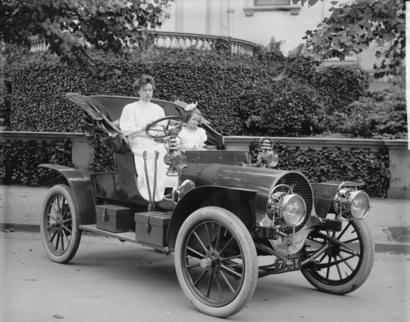
\includegraphics[width=\linewidth]{sample-franklin}
%   \caption{1907 Franklin Model D roadster. Photograph by Harris \&
%     Ewing, Inc. [Public domain], via Wikimedia
%     Commons. (\url{https://goo.gl/VLCRBB}).}
%   \Description{A woman and a girl in white dresses sit in an open car.}
% \end{figure}

% Your figures should contain a caption which describes the figure to
% the reader.

% Figure captions are placed {\itshape below} the figure.

% Every figure should also have a figure description unless it is purely
% decorative. These descriptions convey what’s in the image to someone
% who cannot see it. They are also used by search engine crawlers for
% indexing images, and when images cannot be loaded.

% A figure description must be unformatted plain text less than 2000
% characters long (including spaces).  {\bfseries Figure descriptions
%   should not repeat the figure caption – their purpose is to capture
%   important information that is not already provided in the caption or
%   the main text of the paper.} For figures that convey important and
% complex new information, a short text description may not be
% adequate. More complex alternative descriptions can be placed in an
% appendix and referenced in a short figure description. For example,
% provide a data table capturing the information in a bar chart, or a
% structured list representing a graph.  For additional information
% regarding how best to write figure descriptions and why doing this is
% so important, please see
% \url{https://www.acm.org/publications/taps/describing-figures/}.

% \subsection{The ``Teaser Figure''}

% A ``teaser figure'' is an image, or set of images in one figure, that
% are placed after all author and affiliation information, and before
% the body of the article, spanning the page. If you wish to have such a
% figure in your article, place the command immediately before the
% \verb|\maketitle| command:
% \begin{verbatim}
%   \begin{teaserfigure}
%     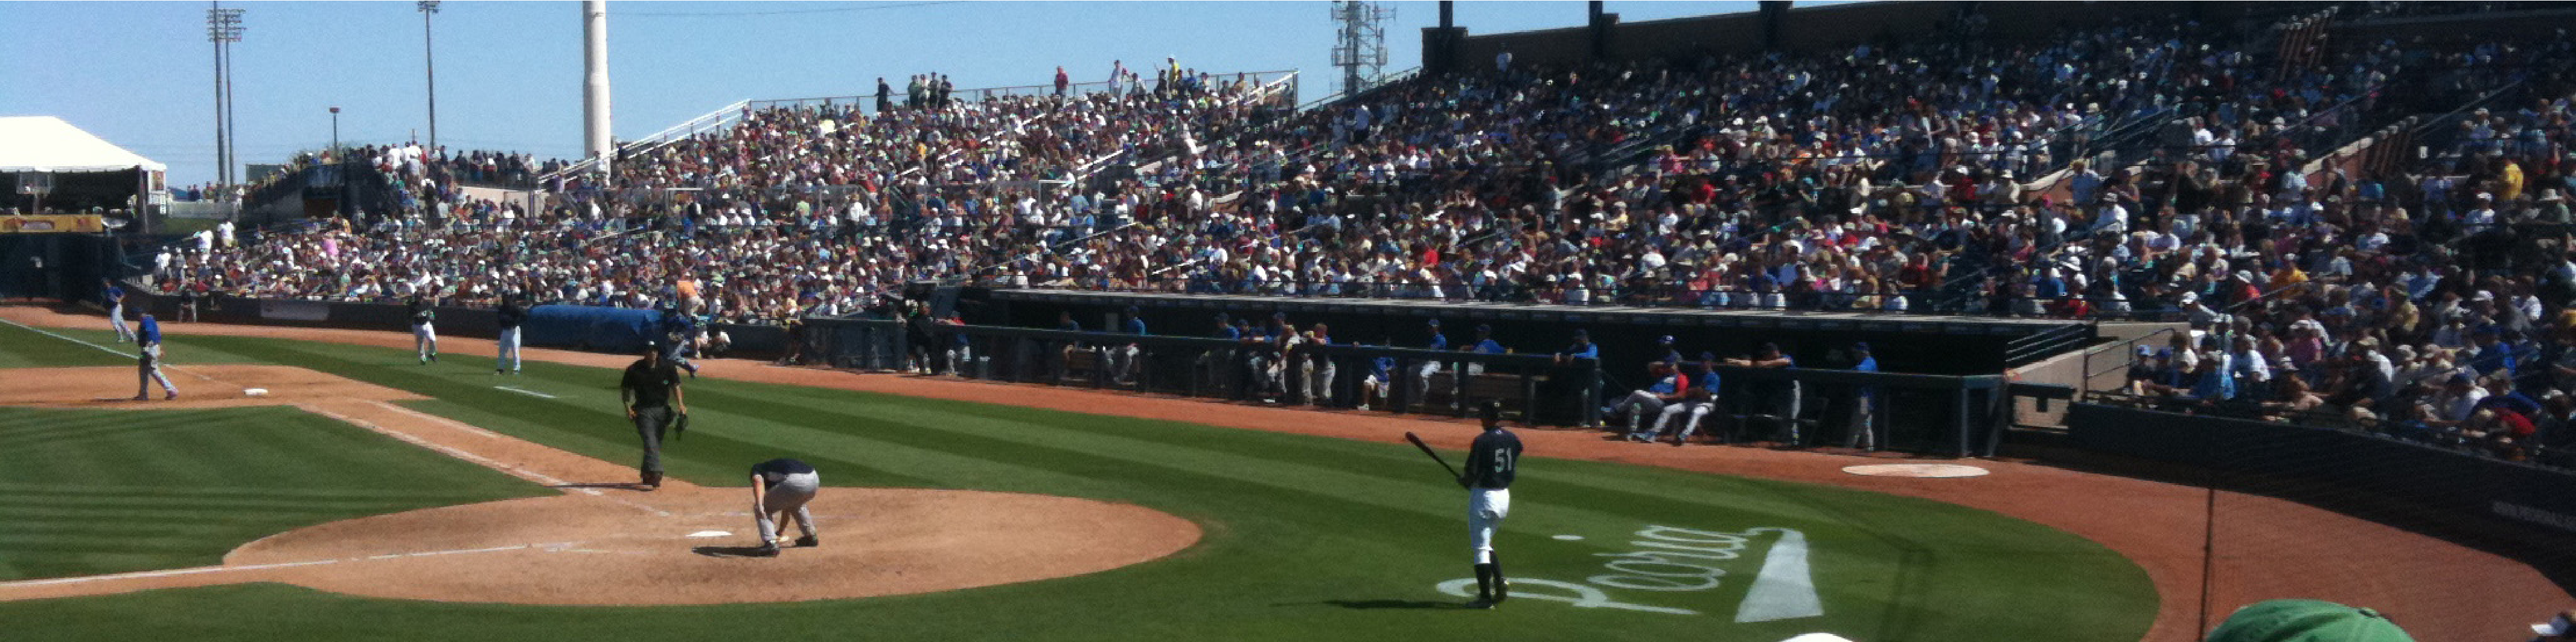
\includegraphics[width=\textwidth]{sampleteaser}
%     \caption{figure caption}
%     \Description{figure description}
%   \end{teaserfigure}
% \end{verbatim}

% \section{Citations and Bibliographies}

% The use of \BibTeX\ for the preparation and formatting of one's
% references is strongly recommended. Authors' names should be complete
% --- use full first names (``Donald E. Knuth'') not initials
% (``D. E. Knuth'') --- and the salient identifying features of a
% reference should be included: title, year, volume, number, pages,
% article DOI, etc.

% The bibliography is included in your source document with these two
% commands, placed just before the \verb|\end{document}| command:
% \begin{verbatim}
%   \bibliographystyle{ACM-Reference-Format}
%   \bibliography{bibfile}
% \end{verbatim}
% where ``\verb|bibfile|'' is the name, without the ``\verb|.bib|''
% suffix, of the \BibTeX\ file.

% Citations and references are numbered by default. A small number of
% ACM publications have citations and references formatted in the
% ``author year'' style; for these exceptions, please include this
% command in the {\bfseries preamble} (before the command
% ``\verb|\begin{document}|'') of your \LaTeX\ source:
% \begin{verbatim}
%   \citestyle{acmauthoryear}
% \end{verbatim}

%   Some examples.  A paginated journal article \cite{Abril07}, an
%   enumerated journal article \cite{Cohen07}, a reference to an entire
%   issue \cite{JCohen96}, a monograph (whole book) \cite{Kosiur01}, a
%   monograph/whole book in a series (see 2a in spec. document)
%   \cite{Harel79}, a divisible-book such as an anthology or compilation
%   \cite{Editor00} followed by the same example, however we only output
%   the series if the volume number is given \cite{Editor00a} (so
%   Editor00a's series should NOT be present since it has no vol. no.),
%   a chapter in a divisible book \cite{Spector90}, a chapter in a
%   divisible book in a series \cite{Douglass98}, a multi-volume work as
%   book \cite{Knuth97}, a couple of articles in a proceedings (of a
%   conference, symposium, workshop for example) (paginated proceedings
%   article) \cite{Andler79, Hagerup1993}, a proceedings article with
%   all possible elements \cite{Smith10}, an example of an enumerated
%   proceedings article \cite{VanGundy07}, an informally published work
%   \cite{Harel78}, a couple of preprints \cite{Bornmann2019,
%     AnzarootPBM14}, a doctoral dissertation \cite{Clarkson85}, a
%   master's thesis: \cite{anisi03}, an online document / world wide web
%   resource \cite{Thornburg01, Ablamowicz07, Poker06}, a video game
%   (Case 1) \cite{Obama08} and (Case 2) \cite{Novak03} and \cite{Lee05}
%   and (Case 3) a patent \cite{JoeScientist001}, work accepted for
%   publication \cite{rous08}, 'YYYYb'-test for prolific author
%   \cite{SaeediMEJ10} and \cite{SaeediJETC10}. Other cites might
%   contain 'duplicate' DOI and URLs (some SIAM articles)
%   \cite{Kirschmer:2010:AEI:1958016.1958018}. Boris / Barbara Beeton:
%   multi-volume works as books \cite{MR781536} and \cite{MR781537}. A
%   couple of citations with DOIs:
%   \cite{2004:ITE:1009386.1010128,Kirschmer:2010:AEI:1958016.1958018}. Online
%   citations: \cite{TUGInstmem, Thornburg01, CTANacmart}. Artifacts:
%   \cite{R} and \cite{UMassCitations}.

% \section{Acknowledgments}

% Identification of funding sources and other support, and thanks to
% individuals and groups that assisted in the research and the
% preparation of the work should be included in an acknowledgment
% section, which is placed just before the reference section in your
% document.

% This section has a special environment:
% \begin{verbatim}
%   \begin{acks}
%   ...
%   \end{acks}
% \end{verbatim}
% so that the information contained therein can be more easily collected
% during the article metadata extraction phase, and to ensure
% consistency in the spelling of the section heading.

% Authors should not prepare this section as a numbered or unnumbered {\verb|\section|}; please use the ``{\verb|acks|}'' environment.

% \section{Appendices}

% If your work needs an appendix, add it before the
% ``\verb|\end{document}|'' command at the conclusion of your source
% document.

% Start the appendix with the ``\verb|appendix|'' command:
% \begin{verbatim}
%   \appendix
% \end{verbatim}
% and note that in the appendix, sections are lettered, not
% numbered. This document has two appendices, demonstrating the section
% and subsection identification method.

% \section{Multi-language papers}

% Papers may be written in languages other than English or include
% titles, subtitles, keywords and abstracts in different languages (as a
% rule, a paper in a language other than English should include an
% English title and an English abstract).  Use \verb|language=...| for
% every language used in the paper.  The last language indicated is the
% main language of the paper.  For example, a French paper with
% additional titles and abstracts in English and German may start with
% the following command
% \begin{verbatim}
% \documentclass[sigconf, language=english, language=german,
%                language=french]{acmart}
% \end{verbatim}

% The title, subtitle, keywords and abstract will be typeset in the main
% language of the paper.  The commands \verb|\translatedXXX|, \verb|XXX|
% begin title, subtitle and keywords, can be used to set these elements
% in the other languages.  The environment \verb|translatedabstract| is
% used to set the translation of the abstract.  These commands and
% environment have a mandatory first argument: the language of the
% second argument.  See \verb|sample-sigconf-i13n.tex| file for examples
% of their usage.

% \section{SIGCHI Extended Abstracts}

% The ``\verb|sigchi-a|'' template style (available only in \LaTeX\ and
% not in Word) produces a landscape-orientation formatted article, with
% a wide left margin. Three environments are available for use with the
% ``\verb|sigchi-a|'' template style, and produce formatted output in
% the margin:
% \begin{itemize}
% \item {\verb|sidebar|}:  Place formatted text in the margin.
% \item {\verb|marginfigure|}: Place a figure in the margin.
% \item {\verb|margintable|}: Place a table in the margin.
% \end{itemize}

% %%
% %% The acknowledgments section is defined using the "acks" environment
% %% (and NOT an unnumbered section). This ensures the proper
% %% identification of the section in the article metadata, and the
% %% consistent spelling of the heading.
% \begin{acks}
% To Robert, for the bagels and explaining CMYK and color spaces.
% \end{acks}

% %%
% %% The next two lines define the bibliography style to be used, and
% %% the bibliography file.
% \bibliographystyle{ACM-Reference-Format}
% \bibliography{sample-base}

% %%
% %% If your work has an appendix, this is the place to put it.
% \appendix

% \section{Research Methods}

% \subsection{Part One}

% Lorem ipsum dolor sit amet, consectetur adipiscing elit. Morbi
% malesuada, quam in pulvinar varius, metus nunc fermentum urna, id
% sollicitudin purus odio sit amet enim. Aliquam ullamcorper eu ipsum
% vel mollis. Curabitur quis dictum nisl. Phasellus vel semper risus, et
% lacinia dolor. Integer ultricies commodo sem nec semper.

% \subsection{Part Two}

% Etiam commodo feugiat nisl pulvinar pellentesque. Etiam auctor sodales
% ligula, non varius nibh pulvinar semper. Suspendisse nec lectus non
% ipsum convallis congue hendrerit vitae sapien. Donec at laoreet
% eros. Vivamus non purus placerat, scelerisque diam eu, cursus
% ante. Etiam aliquam tortor auctor efficitur mattis.

% \section{Online Resources}

% Nam id fermentum dui. Suspendisse sagittis tortor a nulla mollis, in
% pulvinar ex pretium. Sed interdum orci quis metus euismod, et sagittis
% enim maximus. Vestibulum gravida massa ut felis suscipit
% congue. Quisque mattis elit a risus ultrices commodo venenatis eget
% dui. Etiam sagittis eleifend elementum.

% Nam interdum magna at lectus dignissim, ac dignissim lorem
% rhoncus. Maecenas eu arcu ac neque placerat aliquam. Nunc pulvinar
% massa et mattis lacinia.

\end{document}
\endinput
% %%
% %% End of file `sample-sigplan.tex'.
